

% Indicate to rubber that there are external files
% rubber: shell_escape

\documentclass[aspectratio=169]{beamer}


\input{../Latex_Templates/Declare_Mathops}
%\documentclass{beamer}
%%%CHOOSE ASPECT RATIO ABOVE%%%

\usetheme{LU-spfaff}

\usepackage[utf8]{inputenc}
\usepackage[british]{babel}

\title[Cell Reprogramming]{BERN01 - Cell Reprogramming}

\titlecolor{LUIvory} % Choose between LUPink, LULBlue, LUIvory, LUGreen
%\titleimage{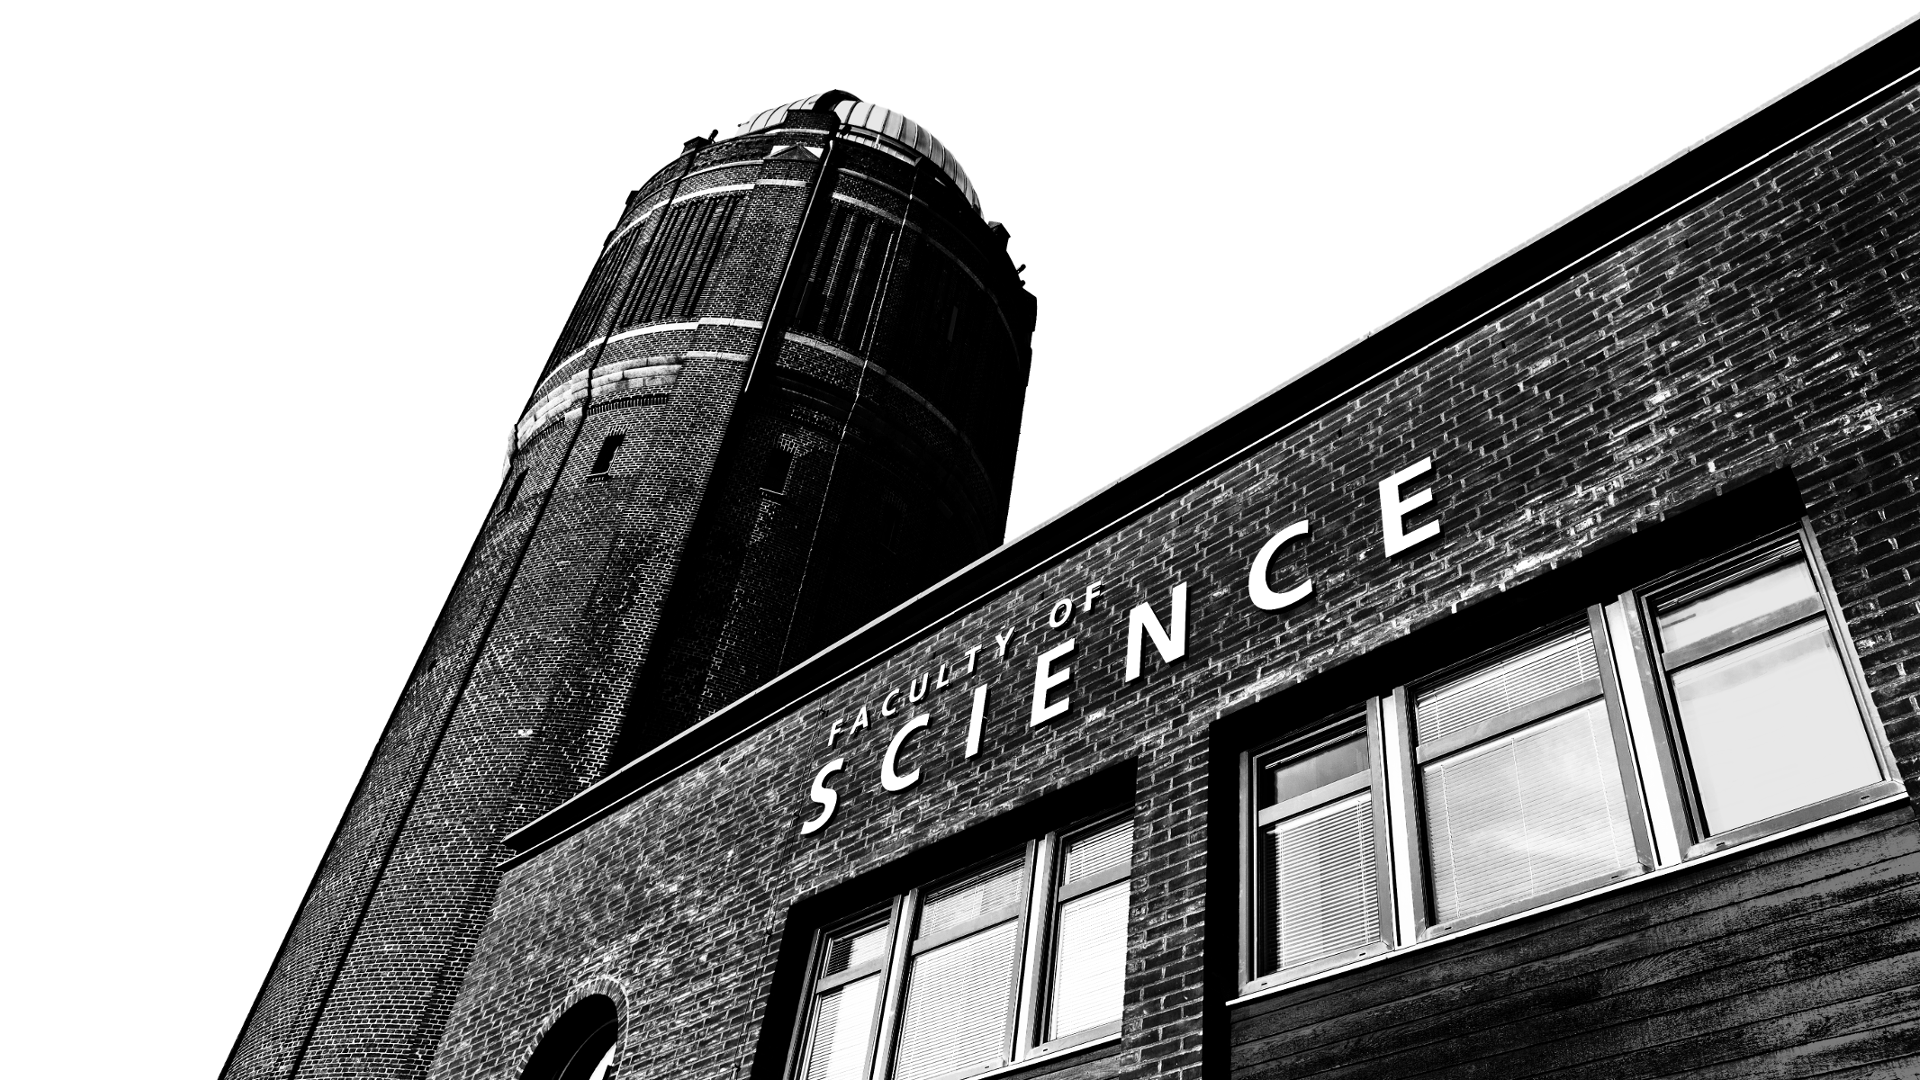
\includegraphics[scale=.5]{astro.png}}
\titleimage{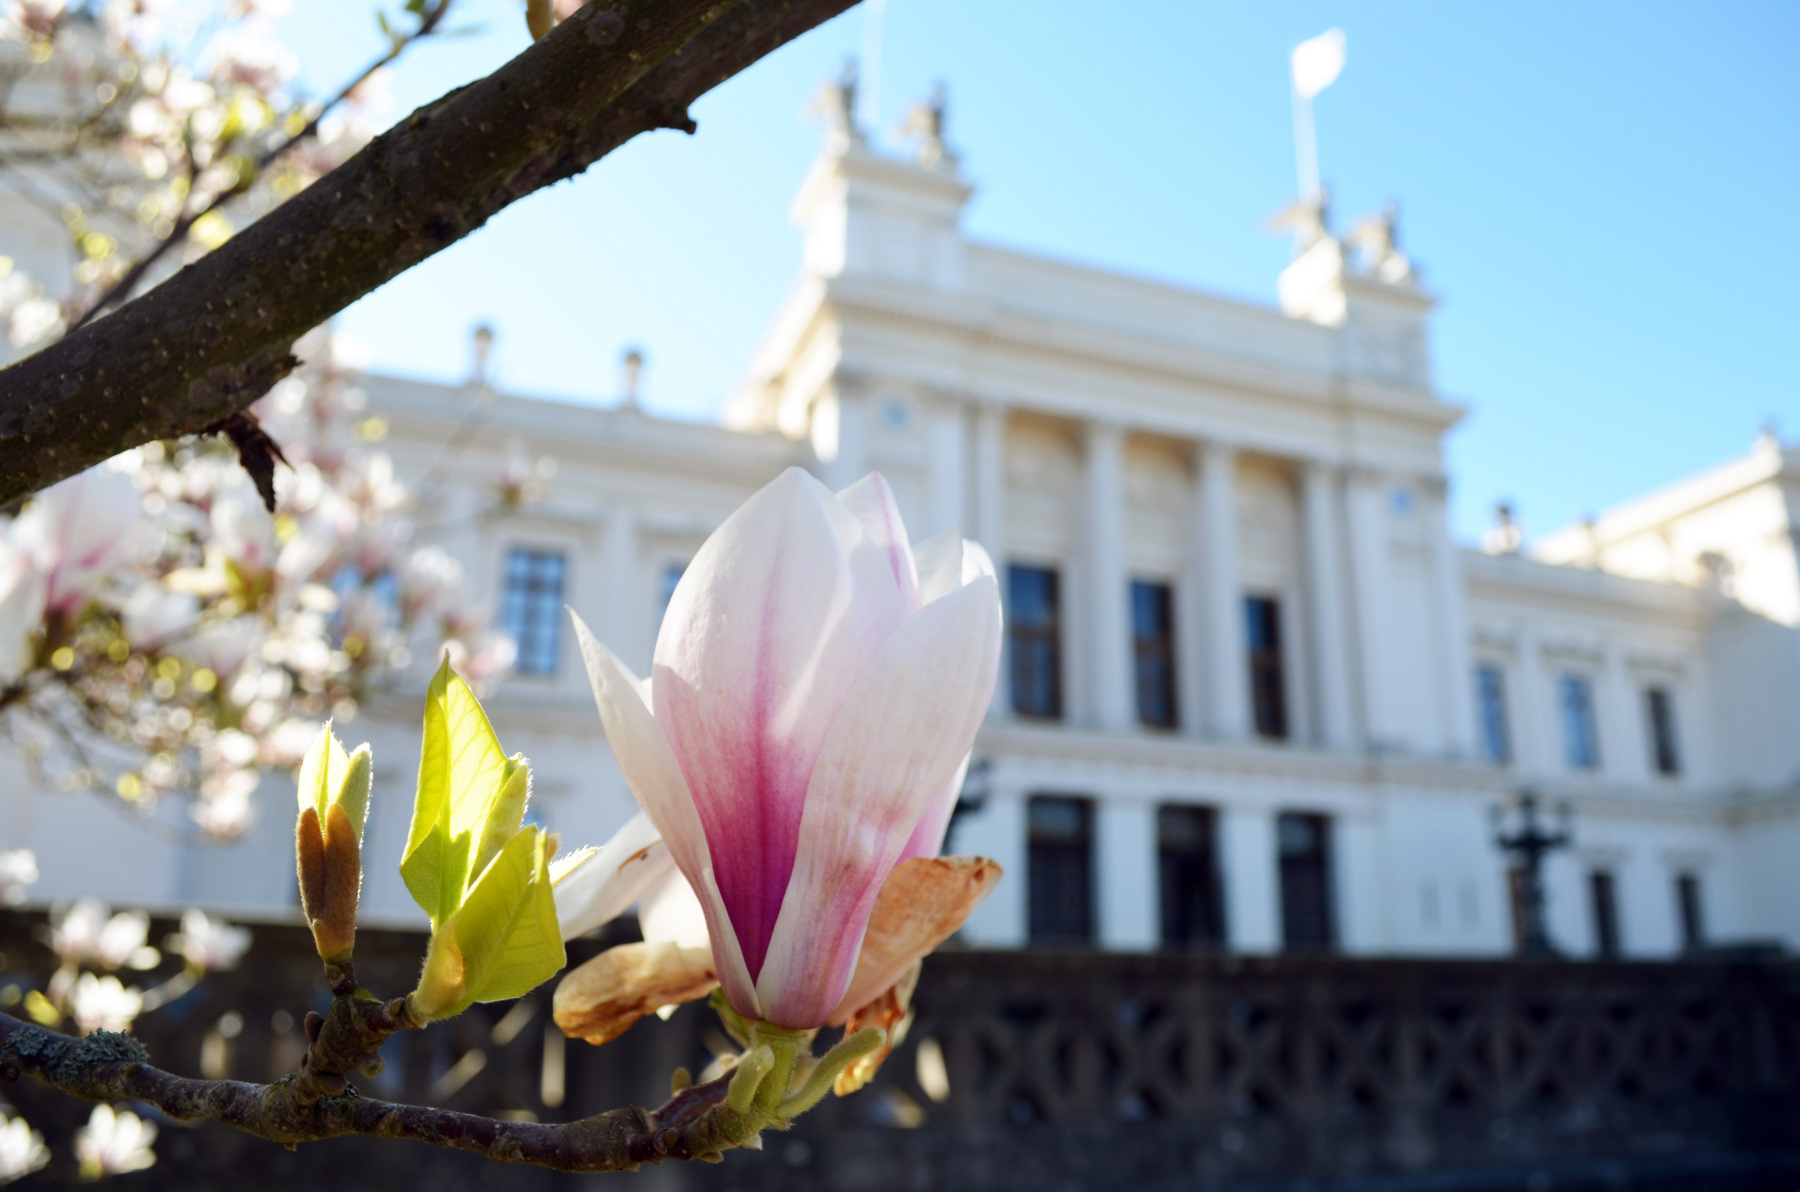
\includegraphics[scale=.6]{lumainb.jpg}}
\author{Gunnarsson, Jimmy \& Koppenhöffer, Theo}
\subtitle{A short experiment on numerical cell reprogramming}
\date{\today}
\institute{Lund University\\Department of Mathematics}

\addbibresource{bibliography.bib}

\begin{document}
% \titleframe{lkj}
\section{Introduction}
\begin{frame}{Introduction}
			\begin{itemize}
				\item Gene expressions and interactions are non-trivial  
				\item Expressions can be modified through complexes and suppression 
				\item Usually governed by some collection of differential equations
			\end{itemize}
\end{frame} 
\begin{frame}{Time evolution}
    \begin{itemize}
        \item Parameters and dynamics 
        \item Expression stages  
        \item Reprogramming 
    \end{itemize}
\end{frame}
\section{Results}
\begin{frame}{Original configuration}

dsff

    
\end{frame}


% \begin{frame}{Plot testing}
% \begin{figure}
%   \centering
%   \graphicspath{{../Plots/}}
%   % This file was created with tikzplotlib v0.10.1.
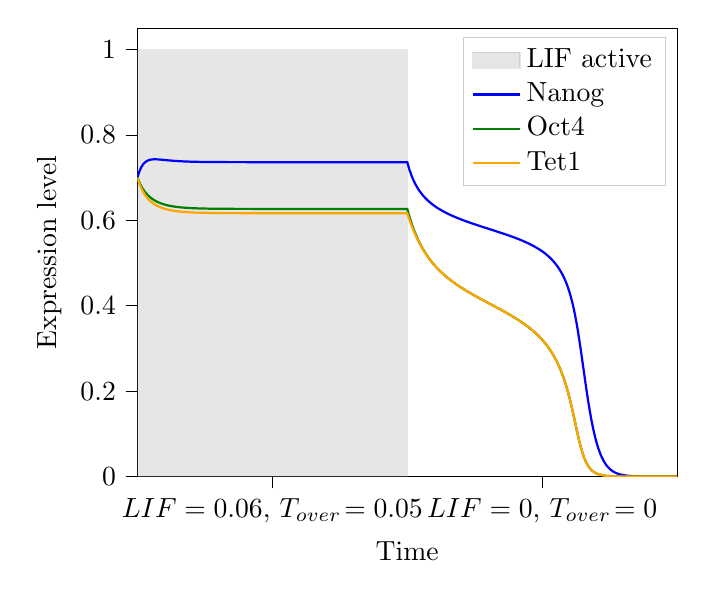
\begin{tikzpicture}

\definecolor{darkgray176}{RGB}{176,176,176}
\definecolor{gray}{RGB}{128,128,128}
\definecolor{green}{RGB}{0,128,0}
\definecolor{lightgray204}{RGB}{204,204,204}
\definecolor{orange}{RGB}{255,165,0}

\begin{axis}[
legend cell align={left},
legend style={fill opacity=0.8, draw opacity=1, text opacity=1, draw=lightgray204},
tick align=outside,
tick pos=left,
x grid style={darkgray176},
xlabel={Time},
xmin=0, xmax=80,
xtick style={color=black},
xtick={20,60},
xticklabels={
  {\(\displaystyle \text{{LIF}}=0.06\), \(\displaystyle T_\text{{over}}\!=0.05\)},
  {\(\displaystyle \text{{LIF}}=0\), \(\displaystyle T_\text{{over}}\!=0\)}
},
y grid style={darkgray176},
ylabel={Expression level},
ymin=0, ymax=1.05,
ytick style={color=black}
]
\path [draw=gray, fill=gray, opacity=0.2]
(axis cs:0,0)
--(axis cs:0,1)
--(axis cs:40,1)
--(axis cs:40,0)
--cycle;
\addlegendimage{area legend, draw=gray, fill=gray, opacity=0.2}
\addlegendentry{LIF active}

\addplot [thick, blue]
table {%
0 0.7
0.2 0.71064370104892
0.4 0.718946240162997
0.6 0.725381606850402
0.8 0.730330465213677
1 0.734098437983533
1.2 0.73693077194489
1.4 0.739024120365422
1.6 0.740536020764474
1.8 0.741592525611385
2 0.742294349779565
2.2 0.742721825129403
2.4 0.742938894651899
2.6 0.742996332652004
2.8 0.742934340850264
3 0.74278464103194
3.2 0.742572161435939
3.4 0.742316395257033
3.6 0.742032494499082
3.8 0.741732150227537
4 0.74142430044295
4.2 0.741115698869126
4.4 0.740811371549437
4.6 0.74051498297573
4.8 0.740229129298086
5 0.739955572789005
5.2 0.739695429008078
5.4 0.739449315908683
5.6 0.73921747234638
5.8 0.738999852008498
5.99999999999999 0.738796197620482
6.19999999999999 0.738606099344073
6.39999999999999 0.738429040522465
6.59999999999999 0.738264433313828
6.79999999999999 0.738111646258821
6.99999999999999 0.737970025427574
7.19999999999999 0.737838910468549
7.39999999999999 0.737717646621138
7.59999999999999 0.737605593543649
7.79999999999999 0.737502131638919
7.99999999999999 0.737406666423302
8.19999999999999 0.737318631374849
8.39999999999999 0.737237489608081
8.59999999999999 0.737162734651619
8.79999999999998 0.737093890547816
8.99999999999998 0.737030511447703
9.19999999999998 0.736972180837762
9.39999999999998 0.736918510505677
9.59999999999998 0.736869139328623
9.79999999999998 0.736823731948922
9.99999999999998 0.736781977386951
10.2 0.736743587629256
10.4 0.736708296220481
10.6 0.736675856880243
10.8 0.736646042160233
11 0.736618642152286
11.2 0.736593463254541
11.4 0.736570327000091
11.6 0.736549068950403
11.8 0.736529537654154
12 0.736511593670979
12.2 0.736495108658685
12.4 0.736479964521899
12.6 0.736466052619666
12.8 0.736453273029212
13 0.736441533862942
13.2 0.736430750635661
13.4 0.736420845678977
13.6 0.736411747599912
13.8 0.736403390780798
14 0.736395714917661
14.2 0.736388664594396
14.4 0.736382188890185
14.6 0.736376241017729
14.8 0.736370777990025
15 0.736365760313547
15.2 0.736361151705825
15.4 0.736356918835565
15.6 0.736353031083559
15.8 0.736349460322776
16 0.736346180716128
16.2 0.73634316853053
16.4 0.736340401965953
16.6 0.736337860998291
16.8 0.736335527234933
17 0.73633338378204
17.2 0.736331415122566
17.4 0.736329607004183
17.6 0.736327946336298
17.8 0.73632642109544
18 0.736325020238332
18.2 0.73632373362203
18.4 0.736322551930565
18.6 0.736321466607544
18.8 0.736320469794247
19 0.736319554272756
19.2 0.73631871341372
19.4 0.736317941128376
19.6 0.736317231824472
19.8 0.736316580365788
20 0.736315982034954
20.2 0.736315432499297
20.4 0.736314927779472
20.6 0.736314464220653
20.8 0.736314038466067
21 0.736313647432692
21.2 0.736313288288929
21.4 0.736312958434105
21.6 0.736312655479636
21.8 0.736312377231733
22 0.736312121675515
22.2 0.736311886960421
22.4 0.736311671386808
22.6000000000001 0.736311473393644
22.8000000000001 0.736311291547202
23.0000000000001 0.73631112453068
23.2000000000001 0.736310971134665
23.4000000000001 0.736310830248376
23.6000000000001 0.736310700851616
23.8000000000001 0.73631058200739
24.0000000000001 0.736310472855118
24.2000000000001 0.736310372604401
24.4000000000001 0.736310280529299
24.6000000000001 0.736310195963075
24.8000000000001 0.736310118293366
25.0000000000001 0.736310046957747
25.2000000000001 0.736309981439663
25.4000000000001 0.736309921264682
25.6000000000001 0.736309865997064
25.8000000000001 0.736309815236607
26.0000000000001 0.736309768615743
26.2000000000001 0.736309725796881
26.4000000000001 0.736309686469961
26.6000000000001 0.736309650350211
26.8000000000001 0.736309617176079
27.0000000000001 0.736309586707347
27.2000000000001 0.736309558723384
27.4000000000001 0.736309533021554
27.6000000000001 0.736309509415745
27.8000000000001 0.736309487735023
28.0000000000001 0.736309467822395
28.2000000000001 0.73630944953367
28.4000000000001 0.736309432736417
28.6000000000001 0.736309417309003
28.8000000000001 0.736309403139716
29.0000000000001 0.736309390125954
29.2000000000001 0.736309378173482
29.4000000000001 0.736309367195751
29.6000000000002 0.736309357113269
29.8000000000002 0.736309347853027
30.0000000000002 0.736309339347971
30.2000000000002 0.736309331536513
30.4000000000002 0.736309324362091
30.6000000000002 0.736309317772753
30.8000000000002 0.736309311720783
31.0000000000002 0.736309306162361
31.2000000000002 0.736309301057235
31.4000000000002 0.736309296368439
31.6000000000002 0.73630929206202
31.8000000000002 0.736309288106796
32.0000000000002 0.736309284474126
32.2000000000002 0.736309281137704
32.4000000000002 0.736309278073373
32.6000000000002 0.736309275258941
32.8000000000002 0.736309272674031
33.0000000000002 0.736309270299923
33.2000000000002 0.736309268119427
33.4000000000002 0.736309266116753
33.6000000000002 0.7363092642774
33.8000000000002 0.736309262588049
34.0000000000002 0.736309261036467
34.2000000000002 0.736309259611418
34.4000000000002 0.736309258302583
34.6000000000002 0.736309257100486
34.8000000000002 0.736309255996422
35.0000000000002 0.736309254982395
35.2000000000002 0.736309254051064
35.4000000000002 0.736309253195684
35.6000000000002 0.736309252410062
35.8000000000002 0.736309251688507
36.0000000000002 0.736309251025797
36.2000000000002 0.736309250417132
36.4000000000002 0.736309249858104
36.6000000000003 0.736309249344665
36.8000000000003 0.736309248873098
37.0000000000003 0.736309248439988
37.2000000000003 0.736309248042199
37.4000000000003 0.73630924767685
37.6000000000003 0.736309247341295
37.8000000000003 0.736309247033106
38.0000000000003 0.73630924675005
38.2000000000003 0.736309246490077
38.4000000000003 0.736309246251306
38.6000000000003 0.736309246032006
38.8000000000003 0.736309245830591
39.0000000000003 0.736309245645602
39.2000000000003 0.736309245475698
39.4000000000003 0.736309245319651
39.6000000000003 0.736309245176329
39.8000000000003 0.736309245044695
40 0.736309244923797
40.1 0.730499077829811
40.3 0.719927114014782
40.5 0.710573203299027
40.7 0.702253427197794
40.9 0.694814486230074
41.1 0.688128368145973
41.3 0.682087963136984
41.5 0.676603456705976
41.7 0.671599361125943
41.9 0.667012071273052
42.1 0.66278785105374
42.3 0.658881173445555
42.5 0.655253350979903
42.7 0.651871404839566
42.9 0.648707130059311
43.1 0.645736321962844
43.3 0.642938135240078
43.5 0.64029455220979
43.7000000000001 0.637789941026187
43.9000000000001 0.635410688040121
44.1000000000001 0.633144891353784
44.3000000000001 0.630982104924262
44.5000000000001 0.628913124469114
44.7000000000001 0.626929807981902
44.9000000000001 0.625024924939778
45.1000000000001 0.623192029329756
45.3000000000001 0.621425352476873
45.5000000000001 0.61971971236033
45.7000000000001 0.618070436680695
45.9000000000001 0.616473297415279
46.1000000000001 0.614924454988475
46.3000000000001 0.613420410504427
46.5000000000001 0.611957964753382
46.7000000000001 0.610534182920594
46.9000000000001 0.609146364106126
47.1000000000001 0.607792014912053
47.3000000000001 0.606468826476057
47.5000000000001 0.605174654431767
47.7000000000001 0.603907501360154
47.9000000000001 0.602665501365969
48.1000000000001 0.601446906471007
48.3000000000001 0.600250074564145
48.5000000000001 0.599073458688095
48.7000000000001 0.597915597476236
48.9000000000001 0.59677510658075
49.1000000000001 0.595650670956584
49.3000000000001 0.594541037885273
49.5000000000001 0.593445010638964
49.7000000000001 0.592361442698705
49.9000000000001 0.591289232452552
50.1000000000001 0.590227318308676
50.3000000000001 0.589174674166775
50.5000000000001 0.588130305197887
50.7000000000002 0.587093243888366
50.9000000000002 0.586062546308565
51.1000000000002 0.585037288570689
51.3000000000002 0.584016563443568
51.5000000000002 0.582999477094728
51.7000000000002 0.581985145932294
51.9000000000002 0.580972693520936
52.1000000000002 0.579961247547277
52.3000000000002 0.578949936811122
52.5000000000002 0.577937888219299
52.7000000000002 0.576924223759159
52.9000000000002 0.575908057428557
53.1000000000002 0.574888492098714
53.3000000000002 0.573864616285508
53.5000000000002 0.572835500803615
53.7000000000002 0.571800195276382
53.9000000000002 0.570757724472407
54.1000000000002 0.569707084437462
54.3000000000002 0.568647238387577
54.5000000000002 0.567577112325729
54.7000000000002 0.566495590340639
54.9000000000002 0.565401509541501
55.1000000000002 0.564293654577045
55.3000000000002 0.563170751680913
55.5000000000002 0.562031462177919
55.7000000000002 0.560874375377042
55.9000000000002 0.559698000766826
56.1000000000002 0.558500759416968
56.3000000000002 0.55728097447593
56.5000000000002 0.556036860638045
56.7000000000002 0.554766512434346
56.9000000000002 0.553467891178682
57.1000000000002 0.552138810373908
57.3000000000002 0.55077691935125
57.5000000000002 0.549379684878349
57.7000000000003 0.547944370426706
57.9000000000003 0.546468012735923
58.1000000000003 0.544947395248208
58.3000000000003 0.543379017910044
58.5000000000003 0.541759062745723
58.7000000000003 0.540083354496233
58.9000000000003 0.538347315482433
59.1000000000003 0.53654591368822
59.3000000000003 0.534673602860784
59.5000000000003 0.532724253182879
59.7000000000003 0.530691070776005
59.9000000000003 0.528566503930868
60.1000000000003 0.526342133516745
60.3000000000003 0.524008544475473
60.5000000000003 0.521555174635468
60.7000000000003 0.518970136259255
60.9000000000003 0.516240004732983
61.1000000000003 0.51334956758423
61.3000000000003 0.510281525541519
61.5000000000003 0.507016135600096
61.7000000000003 0.503530784031565
61.9000000000003 0.499799475019474
62.1000000000003 0.495792218273451
62.3000000000003 0.491474296925766
62.5000000000003 0.486805395971252
62.7000000000003 0.481738572864424
62.9000000000003 0.476219058190889
63.1000000000003 0.470182890117696
63.3000000000003 0.463555419364531
63.5000000000003 0.456249784438824
63.7000000000003 0.448165569308335
63.9000000000003 0.439188044053633
64.1000000000003 0.429188681202705
64.3000000000003 0.418028044026043
64.5000000000003 0.405562592040421
64.7000000000003 0.391657207863928
64.9000000000003 0.376204815674618
65.1000000000003 0.359152640139859
65.3000000000003 0.340531113985326
65.5000000000003 0.320477265525773
65.7000000000002 0.299242575050849
65.9000000000002 0.277178766281155
66.1000000000002 0.254703213744241
66.3000000000002 0.232253631970898
66.5000000000002 0.210244417176737
66.7000000000002 0.189033841504239
66.9000000000002 0.16890559058969
67.1000000000002 0.150063402455317
67.3000000000002 0.132635221891215
67.5000000000001 0.116682954858203
67.7000000000001 0.102214636217407
67.9000000000001 0.0891968420434553
68.1000000000001 0.0775660829172996
68.3000000000001 0.0672385766460131
68.5000000000001 0.0581182250827132
68.7000000000001 0.0501028648330821
68.9000000000001 0.0430889840319757
69.1000000000001 0.0369751436852387
69.3 0.0316643449121116
69.5 0.0270655638235564
69.7 0.0230946464811808
69.9 0.0196747246849033
70.1 0.0167362831014815
70.3 0.0142169812889664
70.5 0.0120613111368607
70.7 0.0102201511313183
70.8999999999999 0.0086502633519355
71.0999999999999 0.0073137667589658
71.2999999999999 0.00617761065202986
71.4999999999999 0.00521306471014694
71.6999999999999 0.00439523634192182
71.8999999999999 0.00370262182435321
72.0999999999999 0.00311669458641709
72.2999999999999 0.0026215317497822
72.4999999999999 0.00220347847111956
72.6999999999998 0.00185084857609898
72.8999999999998 0.00155365930568234
73.0999999999998 0.00130339760987973
73.2999999999998 0.001092815244473
73.4999999999998 0.000915749892222371
73.6999999999998 0.000766969596074491
73.8999999999998 0.000642037923577237
74.0999999999998 0.00053719745364896
74.2999999999998 0.000449269370499412
74.4999999999997 0.000375567151586143
74.6999999999997 0.000313822537759505
74.8999999999997 0.000262122167970111
75.0999999999997 0.000218853444101898
75.2999999999997 0.000182658361319975
75.4999999999997 0.000152394194644519
75.6999999999997 0.000127100072980769
75.8999999999997 0.000105968597829098
76.0999999999997 8.83217760269948e-05
76.2999999999996 7.35906350303933e-05
76.4999999999996 6.12979764483883e-05
76.6999999999996 5.1043799879853e-05
76.8999999999996 4.24929956410269e-05
77.0999999999996 3.53649627635603e-05
77.2999999999996 2.94248586695592e-05
77.4999999999996 2.44762301100998e-05
77.6999999999996 2.03548121254313e-05
77.8999999999996 1.69233137082901e-05
78.0999999999995 1.40670362080046e-05
78.2999999999995 1.16901939092314e-05
78.4999999999995 9.71282619212494e-06
78.6999999999995 8.0682077028342e-06
78.8999999999995 6.70067744800263e-06
79.0999999999995 5.56382003499679e-06
79.2999999999995 4.61894272412345e-06
79.4999999999995 3.83380081129712e-06
79.6999999999994 3.18153135358662e-06
79.8999999999994 2.63976158734856e-06
80 2.40436439063043e-06
};
\addlegendentry{Nanog}
\addplot [thick, green]
table {%
0 0.7
0.2 0.691965561463531
0.4 0.68502204608039
0.6 0.678981058331031
0.8 0.673694649415937
1 0.669044936246984
1.2 0.664936801084228
1.4 0.661292643706171
1.6 0.658048534813955
1.8 0.655151347305733
2 0.652556583695297
2.2 0.650226708135334
2.4 0.648129850226718
2.6 0.646238786823389
2.8 0.644530134481447
3 0.642983703433401
3.2 0.641581976752719
3.4 0.640309687479126
3.6 0.639153473055937
3.8 0.638101591252588
4 0.637143685323932
4.2 0.636270588844821
4.4 0.635474162698075
4.6 0.63474715825729
4.8 0.634083102015055
5 0.633476197849655
5.2 0.632921243863391
5.4 0.632413561310372
5.6 0.631948933596294
5.8 0.6315235537038
5.99999999999999 0.631133978694773
6.19999999999999 0.630777090180769
6.39999999999999 0.630450059846751
6.59999999999999 0.630150319270688
6.79999999999999 0.629875533409693
6.99999999999999 0.62962357722803
7.19999999999999 0.629392515027994
7.39999999999999 0.629180582115061
7.59999999999999 0.628986168486735
7.79999999999999 0.628807804282361
7.99999999999999 0.628644146770946
8.19999999999999 0.628493968686968
8.39999999999999 0.62835614775168
8.59999999999999 0.628229657240422
8.79999999999998 0.62811355747572
8.99999999999998 0.628006988142226
9.19999999999998 0.627909161333223
9.39999999999998 0.627819355250093
9.59999999999998 0.627736908485968
9.79999999999998 0.62766121483329
9.99999999999998 0.627591718562149
10.2 0.62752791012257
10.4 0.627469322229186
10.6 0.627415526291465
10.8 0.627366129156608
11 0.62732077013583
11.2 0.627279118287745
11.4 0.627240869935324
11.6 0.627205746395266
11.8 0.627173491900705
12 0.627143871700065
12.2 0.627116670316521
12.4 0.627091689953987
12.6 0.627068749036903
12.8 0.627047680872229
13 0.627028332423159
13.2 0.62701056318498
13.4 0.62699424415438
13.6 0.626979256884291
13.8 0.626965492617018
14 0.626952851489085
14.2 0.626941241801753
14.4 0.626930579351737
14.6 0.62692078681707
14.8 0.626911793193534
15 0.626903533277456
15.2 0.626895947191004
15.4 0.626888979946476
15.6 0.626882581046352
15.8 0.626876704116155
16 0.626871306567403
16.2 0.626866349288191
16.4 0.62686179635911
16.6 0.626857614792425
16.8 0.626853774292609
17 0.626850247036455
17.2 0.626847007471188
17.4 0.626844032129076
17.6 0.626841299457203
17.8 0.62683878966115
18 0.626836484561458
18.2 0.626834367461809
18.4 0.626832423027982
18.6 0.626830637176695
18.8 0.626828996973517
19 0.626827490539131
19.2 0.626826106963233
19.4 0.626824836225477
19.6 0.626823669122858
19.8 0.626822597203034
20 0.626821612703081
20.2 0.626820708493256
20.4 0.626819878025342
20.6 0.626819115285206
20.8 0.626818414749239
21 0.626817771344341
21.2 0.626817180411169
21.4 0.626816637670394
21.6 0.626816139191703
21.8 0.626815681365328
22 0.626815260875907
22.2 0.626814874678464
22.4 0.626814519976364
22.6000000000001 0.626814194201052
22.8000000000001 0.626813894993453
23.0000000000001 0.626813620186886
23.2000000000001 0.626813367791375
23.4000000000001 0.626813135979234
23.6000000000001 0.626812923071833
23.8000000000001 0.626812727527442
24.0000000000001 0.626812547930064
24.2000000000001 0.626812382979182
24.4000000000001 0.626812231480339
24.6000000000001 0.626812092336493
24.8000000000001 0.626811964540067
25.0000000000001 0.626811847165655
25.2000000000001 0.62681173936332
25.4000000000001 0.626811640352441
25.6000000000001 0.626811549416058
25.8000000000001 0.626811465895681
26.0000000000001 0.62681138918652
26.2000000000001 0.62681131873311
26.4000000000001 0.626811254025282
26.6000000000001 0.626811194594476
26.8000000000001 0.62681114001034
27.0000000000001 0.626811089877621
27.2000000000001 0.626811043833298
27.4000000000001 0.626811001543957
27.6000000000001 0.626810962703373
27.8000000000001 0.626810927030294
28.0000000000001 0.626810894266405
28.2000000000001 0.626810864174458
28.4000000000001 0.626810836536551
28.6000000000001 0.626810811152554
28.8000000000001 0.626810787838658
29.0000000000001 0.626810766426042
29.2000000000001 0.626810746759655
29.4000000000001 0.626810728697088
29.6000000000002 0.626810712107549
29.8000000000002 0.626810696870909
30.0000000000002 0.626810682876838
30.2000000000002 0.626810670024003
30.4000000000002 0.626810658219333
30.6000000000002 0.626810647377351
30.8000000000002 0.626810637419547
31.0000000000002 0.626810628273815
31.2000000000002 0.62681061987393
31.4000000000002 0.626810612159067
31.6000000000002 0.626810605073362
31.8000000000002 0.626810598565505
32.0000000000002 0.626810592588372
32.2000000000002 0.626810587098683
32.4000000000002 0.626810582056685
32.6000000000002 0.626810577425869
32.8000000000002 0.626810573172702
33.0000000000002 0.626810569266387
33.2000000000002 0.626810565678637
33.4000000000002 0.626810562383472
33.6000000000002 0.626810559357033
33.8000000000002 0.626810556577404
34.0000000000002 0.626810554024457
34.2000000000002 0.626810551679706
34.4000000000002 0.626810549526173
34.6000000000002 0.626810547548264
34.8000000000002 0.626810545731656
35.0000000000002 0.626810544063194
35.2000000000002 0.626810542530798
35.4000000000002 0.62681054112337
35.6000000000002 0.62681053983072
35.8000000000002 0.626810538643488
36.0000000000002 0.626810537553076
36.2000000000002 0.626810536551588
36.4000000000002 0.626810535631773
36.6000000000003 0.626810534786971
36.8000000000003 0.626810534011063
37.0000000000003 0.626810533298431
37.2000000000003 0.626810532643915
37.4000000000003 0.626810532042776
37.6000000000003 0.626810531490661
37.8000000000003 0.626810530983571
38.0000000000003 0.626810530517836
38.2000000000003 0.626810530090081
38.4000000000003 0.626810529697211
38.6000000000003 0.626810529336379
38.8000000000003 0.626810529004974
39.0000000000003 0.626810528700596
39.2000000000003 0.62681052842104
39.4000000000003 0.626810528164282
39.6000000000003 0.626810527928463
39.8000000000003 0.626810527711875
40 0.626810527512951
40.1 0.620932021388433
40.3 0.609862817457274
40.5 0.599627150591179
40.7 0.590136516464879
40.9 0.581313886508895
41.1 0.573091923387776
41.3 0.565411525682923
41.5 0.558220631599366
41.7 0.55147322791217
41.9 0.545128522838645
42.1 0.539150250957346
42.3 0.53350608541793
42.5 0.528167138067734
42.7 0.523107532200184
42.9 0.518304035738703
43.1 0.513735745055604
43.3 0.509383811471943
43.5 0.505231203927036
43.7000000000001 0.501262502444509
43.9000000000001 0.497463717928819
44.1000000000001 0.493822134555997
44.3000000000001 0.490326171614989
44.5000000000001 0.4869652621414
44.7000000000001 0.483729746085965
44.9000000000001 0.480610776093006
45.1000000000001 0.477600234242396
45.3000000000001 0.474690658342446
45.5000000000001 0.471875176558611
45.7000000000001 0.469147449330273
45.9000000000001 0.466501617670221
46.1000000000001 0.463932257062911
46.3000000000001 0.461434336281425
46.5000000000001 0.459003180532124
46.7000000000001 0.456634438412466
46.9000000000001 0.454324052233301
47.1000000000001 0.45206823131369
47.3000000000001 0.449863427905335
47.5000000000001 0.447706315446035
47.7000000000001 0.445593768878296
47.9000000000001 0.443522846801028
48.1000000000001 0.441490775249857
48.3000000000001 0.43949493292557
48.5000000000001 0.437532837711077
48.7000000000001 0.435602134335423
48.9000000000001 0.43370058305922
49.1000000000001 0.431826049269638
49.3000000000001 0.429976493885141
49.5000000000001 0.42814996448061
49.7000000000001 0.426344587052672
49.9000000000001 0.424558558352986
50.1000000000001 0.422790138724195
50.3000000000001 0.421037645379258
50.5000000000001 0.419299446070098
50.7000000000002 0.417573953095993
50.9000000000002 0.415859617606011
51.1000000000002 0.414154924153045
51.3000000000002 0.412458385459785
51.5000000000002 0.410768537359223
51.7000000000002 0.409083933874134
51.9000000000002 0.407403142401401
52.1000000000002 0.405724738968058
52.3000000000002 0.404047303526602
52.5000000000002 0.402369415257395
52.7000000000002 0.400689647845877
52.9000000000002 0.399006564701898
53.1000000000002 0.397318714087577
53.3000000000002 0.395624624118939
53.5000000000002 0.393922797604859
53.7000000000002 0.392211706684801
53.9000000000002 0.390489787224191
54.1000000000002 0.388755432923205
54.3000000000002 0.387006989090946
54.5000000000002 0.385242746032671
54.7000000000002 0.383460931992545
54.9000000000002 0.381659705588413
55.1000000000002 0.37983714766814
55.3000000000002 0.377991252509006
55.5000000000002 0.376119918272289
55.7000000000002 0.374220936614419
55.9000000000002 0.372291981343566
56.1000000000002 0.370330595996127
56.3000000000002 0.36833418019088
56.5000000000002 0.366299974599241
56.7000000000002 0.364225044347703
56.9000000000002 0.362106260642588
57.1000000000002 0.359940280377174
57.3000000000002 0.357723523446347
57.5000000000002 0.355452147453388
57.7000000000003 0.353122019446424
57.9000000000003 0.350728684267385
58.1000000000003 0.3482673290328
58.3000000000003 0.345732743192077
58.5000000000003 0.343119273523608
58.7000000000003 0.340420773330396
58.9000000000003 0.337630544983431
59.1000000000003 0.334741274831099
59.3000000000003 0.331744959345357
59.5000000000003 0.328632821209717
59.7000000000003 0.325395213871203
59.9000000000003 0.322021512881634
60.1000000000003 0.318499992150228
60.3000000000003 0.314817683033752
60.5000000000003 0.310960214027212
60.7000000000003 0.306911628729938
60.9000000000003 0.302654179819182
61.1000000000003 0.298168097080356
61.3000000000003 0.293431328303532
61.5000000000003 0.288419253352041
61.7000000000003 0.283104374402488
61.9000000000003 0.277455989969392
62.1000000000003 0.271439867984876
62.3000000000003 0.265017945627868
62.5000000000003 0.258148103386819
62.7000000000003 0.25078409180883
62.9000000000003 0.242875736885623
63.1000000000003 0.234369620969652
63.3000000000003 0.225210538021468
63.5000000000003 0.215344159412326
63.7000000000003 0.204721511594379
63.9000000000003 0.193306018710915
64.1000000000003 0.181083889354457
64.3000000000003 0.168078290965753
64.5000000000003 0.15436667162521
64.7000000000003 0.140098352479502
64.9000000000003 0.125506216770131
65.1000000000003 0.11090349363388
65.3000000000003 0.0966576988785754
65.5000000000003 0.0831419028252794
65.7000000000002 0.0706764133968556
65.9000000000002 0.0594821616571918
66.1000000000002 0.0496620583741006
66.3000000000002 0.0412116841746364
66.5000000000002 0.0340480402104666
66.7000000000002 0.0280422768442586
66.9000000000002 0.0230470079847357
67.1000000000002 0.0189149405947334
67.3000000000002 0.0155095234871211
67.5000000000001 0.0127098038154676
67.7000000000001 0.0104116766913357
67.9000000000001 0.00852716702800754
68.1000000000001 0.00698279958300663
68.3000000000001 0.0057176684921081
68.5000000000001 0.00468152704500899
68.7000000000001 0.00383304604497188
68.9000000000001 0.00313829418483346
69.1000000000001 0.00256944542954618
69.3 0.0021036960983811
69.5 0.00172236596080566
69.7 0.00141015624717435
69.9 0.00115453925075585
70.1 0.000945257196509206
70.3 0.000773911305960235
70.5 0.000633625056629029
70.7 0.000518768348758541
70.8999999999999 0.000424731612780637
71.0999999999999 0.00034774083812427
71.2999999999999 0.000284706120351706
71.4999999999999 0.000233097657230241
71.6999999999999 0.00019084422087068
71.8999999999999 0.000156250032895658
72.0999999999999 0.000127926707232102
72.2999999999999 0.000104737529438197
72.4999999999999 8.57518364160456e-05
72.6999999999998 7.02076656556964e-05
72.8999999999998 5.74811750130168e-05
73.0999999999998 4.70616057375755e-05
73.2999999999998 3.85307839320765e-05
73.4999999999998 3.15463377661938e-05
73.6999999999998 2.582795689317e-05
73.8999999999998 2.11461426115198e-05
74.0999999999998 1.73129972764077e-05
74.2999999999998 1.41746833074689e-05
74.4999999999997 1.16052491465947e-05
74.6999999999997 9.50157437969476e-06
74.8999999999997 7.77923115242739e-06
75.0999999999997 6.36909578398107e-06
75.2999999999997 5.21457459107222e-06
75.4999999999997 4.26933258473614e-06
75.6999999999997 3.49543388453897e-06
75.8999999999997 2.86181921850399e-06
76.0999999999997 2.34305940547893e-06
76.2999999999996 1.91833479281515e-06
76.4999999999996 1.57059969060961e-06
76.6999999999996 1.28589826832208e-06
76.8999999999996 1.05280445829703e-06
77.0999999999996 8.61963387551961e-07
77.2999999999996 7.05715933879939e-07
77.4999999999996 5.77791338384441e-07
77.6999999999996 4.73055537908372e-07
77.8999999999996 3.8730511705401e-07
78.0999999999995 3.17098610365018e-07
78.2999999999995 2.59618384234782e-07
78.4999999999995 2.12557555377148e-07
78.6999999999995 1.74027407500737e-07
78.8999999999995 1.42481590492942e-07
79.0999999999995 1.16654059960712e-07
79.2999999999995 9.55082664240166e-08
79.4999999999995 7.81955549459063e-08
79.6999999999994 6.40211056302942e-08
79.8999999999994 5.24160480600293e-08
80 4.74280016058462e-08
};
\addlegendentry{Oct4}
\addplot [thick, orange]
table {%
0 0.7
0.2 0.690152868999692
0.4 0.681725246549559
0.6 0.674469174702793
0.8 0.668187939068922
1 0.662723730670789
1.2 0.657948743215229
1.4 0.653758613356933
1.6 0.650067500004518
1.8 0.646804336197728
2 0.643909936536559
2.2 0.641334739726968
2.4 0.639037029766767
2.6 0.636981522611879
2.8 0.635138235113295
3 0.633481574121988
3.2 0.631989598796789
3.4 0.630643420182459
3.6 0.629426710283642
3.8 0.628325298973943
4 0.627326841715227
4.2 0.626420544615096
4.4 0.625596936098881
4.6 0.624847676616256
4.8 0.624165399486844
5 0.623543577320753
5.2 0.622976409508541
5.4 0.622458727120599
5.6 0.621985912234139
5.8 0.62155382925183
5.99999999999999 0.621158766217028
6.19999999999999 0.620797384487545
6.39999999999999 0.620466675419832
6.59999999999999 0.620163922951358
6.79999999999999 0.61988667116142
6.99999999999999 0.619632696047896
7.19999999999999 0.619399980886254
7.39999999999999 0.619186694642821
7.59999999999999 0.618991173001194
7.79999999999999 0.618811901632256
7.99999999999999 0.618647501397314
8.19999999999999 0.618496715222742
8.39999999999999 0.618358396424984
8.59999999999999 0.618231498298411
8.79999999999998 0.618115064806515
8.99999999999998 0.618008222240303
9.19999999999998 0.617910171727272
9.39999999999998 0.617820182490774
9.59999999999998 0.617737585773354
9.79999999999998 0.617661769349302
9.99999999999998 0.617592172561462
10.2 0.617528281825769
10.4 0.617469626554027
10.6 0.617415775451571
10.8 0.617366333151649
11 0.617320937152844
11.2 0.617279255029711
11.4 0.617240981890176
11.6 0.617205838056147
11.8 0.617173566946287
12 0.617143933142191
12.2 0.617116720621079
12.4 0.617091731139876
12.6 0.617068782757056
12.8 0.617047708479955
13 0.617028355026454
13.2 0.617010581690992
13.4 0.616994259305822
13.6 0.616979269289242
13.8 0.616965502773333
14 0.616952859804372
14.2 0.616941248609735
14.4 0.616930584925641
14.6 0.616920791380596
14.8 0.616911796929833
15 0.616903536336479
15.2 0.61689594969552
15.4 0.616888981997
15.6 0.61688258272518
15.8 0.616876705490663
16 0.616871307692755
16.2 0.616866350209551
16.4 0.616861797113455
16.6 0.616857615410031
16.8 0.616853774798262
17 0.616850247450449
17.2 0.616847007810138
17.4 0.616844032406585
17.6 0.616841299684407
17.8 0.616838789847169
18 0.616836484713758
18.2 0.616834367586502
18.4 0.616832423130072
18.6 0.616830637260279
18.8 0.61682899704195
19 0.616827490595159
19.2 0.616826107009105
19.4 0.616824836263034
19.6 0.616823669153607
19.8 0.616822597228209
20 0.616821612723693
20.2 0.616820708510132
20.4 0.616819878039158
20.6 0.616819115296518
20.8 0.616818414758501
21 0.616817771351923
21.2 0.616817180417377
21.4 0.616816637675477
21.6 0.616816139195864
21.8 0.616815681368735
22 0.616815260878696
22.2 0.616814874680748
22.4 0.616814519978234
22.6000000000001 0.616814194202583
22.8000000000001 0.616813894994706
23.0000000000001 0.616813620187912
23.2000000000001 0.616813367792215
23.4000000000001 0.616813135979922
23.6000000000001 0.616812923072396
23.8000000000001 0.616812727527903
24.0000000000001 0.616812547930442
24.2000000000001 0.616812382979491
24.4000000000001 0.616812231480592
24.6000000000001 0.616812092336701
24.8000000000001 0.616811964540237
25.0000000000001 0.616811847165794
25.2000000000001 0.616811739363434
25.4000000000001 0.616811640352534
25.6000000000001 0.616811549416134
25.8000000000001 0.616811465895743
26.0000000000001 0.616811389186572
26.2000000000001 0.616811318733152
26.4000000000001 0.616811254025317
26.6000000000001 0.616811194594504
26.8000000000001 0.616811140010363
27.0000000000001 0.61681108987764
27.2000000000001 0.616811043833314
27.4000000000001 0.61681100154397
27.6000000000001 0.616810962703383
27.8000000000001 0.616810927030302
28.0000000000001 0.616810894266412
28.2000000000001 0.616810864174463
28.4000000000001 0.616810836536556
28.6000000000001 0.616810811152558
28.8000000000001 0.616810787838661
29.0000000000001 0.616810766426045
29.2000000000001 0.616810746759657
29.4000000000001 0.61681072869709
29.6000000000002 0.61681071210755
29.8000000000002 0.61681069687091
30.0000000000002 0.616810682876839
30.2000000000002 0.616810670024004
30.4000000000002 0.616810658219334
30.6000000000002 0.616810647377352
30.8000000000002 0.616810637419547
31.0000000000002 0.616810628273815
31.2000000000002 0.61681061987393
31.4000000000002 0.616810612159067
31.6000000000002 0.616810605073362
31.8000000000002 0.616810598565505
32.0000000000002 0.616810592588372
32.2000000000002 0.616810587098683
32.4000000000002 0.616810582056685
32.6000000000002 0.616810577425869
32.8000000000002 0.616810573172702
33.0000000000002 0.616810569266387
33.2000000000002 0.616810565678637
33.4000000000002 0.616810562383472
33.6000000000002 0.616810559357033
33.8000000000002 0.616810556577404
34.0000000000002 0.616810554024457
34.2000000000002 0.616810551679706
34.4000000000002 0.616810549526173
34.6000000000002 0.616810547548264
34.8000000000002 0.616810545731656
35.0000000000002 0.616810544063194
35.2000000000002 0.616810542530798
35.4000000000002 0.61681054112337
35.6000000000002 0.616810539830721
35.8000000000002 0.616810538643488
36.0000000000002 0.616810537553076
36.2000000000002 0.616810536551588
36.4000000000002 0.616810535631774
36.6000000000003 0.616810534786971
36.8000000000003 0.616810534011063
37.0000000000003 0.616810533298431
37.2000000000003 0.616810532643915
37.4000000000003 0.616810532042776
37.6000000000003 0.616810531490661
37.8000000000003 0.616810530983572
38.0000000000003 0.616810530517836
38.2000000000003 0.616810530090081
38.4000000000003 0.616810529697211
38.6000000000003 0.616810529336379
38.8000000000003 0.616810529004974
39.0000000000003 0.616810528700596
39.2000000000003 0.61681052842104
39.4000000000003 0.616810528164282
39.6000000000003 0.616810527928463
39.8000000000003 0.616810527711875
40 0.616810527512951
40.1 0.6118836472051
40.3 0.602454635243153
40.5 0.593561843984086
40.7 0.585170663415541
40.9 0.577248189899463
41.1 0.569763212538762
41.3 0.56268620774094
41.5 0.555989329986882
41.7 0.549646392661436
41.9 0.543632836637079
42.1 0.537925686666365
42.3 0.532503496973123
42.5 0.527346288074751
42.7 0.522435477066823
42.9 0.517753803532895
43.1 0.513285253027079
43.3 0.50901497979393
43.5 0.504929230089339
43.7000000000001 0.501015267176799
43.9000000000001 0.497261298811767
44.1000000000001 0.493656407799746
44.3000000000001 0.49019048602295
44.5000000000001 0.486854172174375
44.7000000000001 0.483638793313543
44.9000000000001 0.480536310261097
45.1000000000001 0.477539266775719
45.3000000000001 0.474640742402507
45.5000000000001 0.471834308843488
45.7000000000001 0.469113989675071
45.9000000000001 0.466474223221502
46.1000000000001 0.463909828385267
46.3000000000001 0.461415973233274
46.5000000000001 0.458988146139873
46.7000000000001 0.456622129293168
46.9000000000001 0.454313974378782
47.1000000000001 0.452059980264265
47.3000000000001 0.449856672517421
47.5000000000001 0.447700784602198
47.7000000000001 0.445589240606352
47.9000000000001 0.443519139365527
48.1000000000001 0.441487739858395
48.3000000000001 0.439492447757231
48.5000000000001 0.43753080302733
48.7000000000001 0.435600468477266
48.9000000000001 0.433699219169915
49.1000000000001 0.43182493261152
49.3000000000001 0.429975579642798
49.5000000000001 0.428149215962288
49.7000000000001 0.426343974217702
49.9000000000001 0.424558056606149
50.1000000000001 0.422789727928629
50.3000000000001 0.421037309048295
50.5000000000001 0.419299170705595
50.7000000000002 0.417573727646606
50.9000000000002 0.415859433023664
51.1000000000002 0.414154773029801
51.3000000000002 0.412458261730538
51.5000000000002 0.410768436058283
51.7000000000002 0.409083850935939
51.9000000000002 0.40740307449735
52.1000000000002 0.405724683372923
52.3000000000002 0.404047258009156
52.5000000000002 0.402369377990861
52.7000000000002 0.400689617334621
52.9000000000002 0.399006539721393
53.1000000000002 0.39731869363527
53.3000000000002 0.395624607374006
53.5000000000002 0.393922783895268
53.7000000000002 0.392211695460336
53.9000000000002 0.390489778034378
54.1000000000002 0.388755425399222
54.3000000000002 0.387006982930829
54.5000000000002 0.385242740989194
54.7000000000002 0.383460927863296
54.9000000000002 0.381659702207669
55.1000000000002 0.379837144900221
55.3000000000002 0.377991250242825
55.5000000000002 0.376119916416897
55.7000000000002 0.374220935095353
55.9000000000002 0.37229198009986
56.1000000000002 0.370330594977866
56.3000000000002 0.368334179357199
56.5000000000002 0.366299973916681
56.7000000000002 0.36422504378887
56.9000000000002 0.362106260185054
57.1000000000002 0.359940280002576
57.3000000000002 0.357723523139653
57.5000000000002 0.355452147202288
57.7000000000003 0.35312201924084
57.9000000000003 0.350728684099068
58.1000000000003 0.348267328894993
58.3000000000003 0.34573274307925
58.5000000000003 0.343119273431234
58.7000000000003 0.340420773254767
58.9000000000003 0.33763054492151
59.1000000000003 0.334741274780402
59.3000000000003 0.33174495930385
59.5000000000003 0.328632821175734
59.7000000000003 0.32539521384338
59.9000000000003 0.322021512858855
60.1000000000003 0.318499992131578
60.3000000000003 0.314817683018483
60.5000000000003 0.310960214014711
60.7000000000003 0.306911628719703
60.9000000000003 0.302654179810802
61.1000000000003 0.298168097073495
61.3000000000003 0.293431328297915
61.5000000000003 0.288419253347442
61.7000000000003 0.283104374398723
61.9000000000003 0.277455989966309
62.1000000000003 0.271439867982352
62.3000000000003 0.265017945625801
62.5000000000003 0.258148103385128
62.7000000000003 0.250784091807445
62.9000000000003 0.242875736884489
63.1000000000003 0.234369620968723
63.3000000000003 0.225210538020708
63.5000000000003 0.215344159411703
63.7000000000003 0.20472151159387
63.9000000000003 0.193306018710498
64.1000000000003 0.181083889354115
64.3000000000003 0.168078290965473
64.5000000000003 0.154366671624981
64.7000000000003 0.140098352479314
64.9000000000003 0.125506216769977
65.1000000000003 0.110903493633755
65.3000000000003 0.0966576988784725
65.5000000000003 0.0831419028251951
65.7000000000002 0.0706764133967866
65.9000000000002 0.0594821616571353
66.1000000000002 0.0496620583740543
66.3000000000002 0.0412116841745985
66.5000000000002 0.0340480402104356
66.7000000000002 0.0280422768442332
66.9000000000002 0.0230470079847149
67.1000000000002 0.0189149405947164
67.3000000000002 0.0155095234871072
67.5000000000001 0.0127098038154561
67.7000000000001 0.0104116766913264
67.9000000000001 0.0085271670279999
68.1000000000001 0.00698279958300038
68.3000000000001 0.00571766849210297
68.5000000000001 0.00468152704500479
68.7000000000001 0.00383304604496845
68.9000000000001 0.00313829418483064
69.1000000000001 0.00256944542954387
69.3 0.00210369609837921
69.5 0.00172236596080412
69.7 0.00141015624717309
69.9 0.00115453925075482
70.1 0.000945257196508359
70.3 0.000773911305959541
70.5 0.000633625056628461
70.7 0.000518768348758075
70.8999999999999 0.000424731612780256
71.0999999999999 0.000347740838123958
71.2999999999999 0.000284706120351451
71.4999999999999 0.000233097657230032
71.6999999999999 0.000190844220870508
71.8999999999999 0.000156250032895518
72.0999999999999 0.000127926707231988
72.2999999999999 0.000104737529438103
72.4999999999999 8.57518364159687e-05
72.6999999999998 7.02076656556334e-05
72.8999999999998 5.74811750129653e-05
73.0999999999998 4.70616057375333e-05
73.2999999999998 3.8530783932042e-05
73.4999999999998 3.15463377661656e-05
73.6999999999998 2.58279568931468e-05
73.8999999999998 2.11461426115009e-05
74.0999999999998 1.73129972763922e-05
74.2999999999998 1.41746833074562e-05
74.4999999999997 1.16052491465843e-05
74.6999999999997 9.50157437968624e-06
74.8999999999997 7.77923115242041e-06
75.0999999999997 6.36909578397536e-06
75.2999999999997 5.21457459106754e-06
75.4999999999997 4.26933258473231e-06
75.6999999999997 3.49543388453583e-06
75.8999999999997 2.86181921850142e-06
76.0999999999997 2.34305940547682e-06
76.2999999999996 1.91833479281343e-06
76.4999999999996 1.5705996906082e-06
76.6999999999996 1.28589826832093e-06
76.8999999999996 1.05280445829609e-06
77.0999999999996 8.61963387551187e-07
77.2999999999996 7.05715933879305e-07
77.4999999999996 5.77791338383922e-07
77.6999999999996 4.73055537907948e-07
77.8999999999996 3.87305117053663e-07
78.0999999999995 3.17098610364733e-07
78.2999999999995 2.59618384234549e-07
78.4999999999995 2.12557555376957e-07
78.6999999999995 1.74027407500581e-07
78.8999999999995 1.42481590492814e-07
79.0999999999995 1.16654059960608e-07
79.2999999999995 9.55082664239309e-08
79.4999999999995 7.81955549458361e-08
79.6999999999994 6.40211056302368e-08
79.8999999999994 5.24160480599823e-08
80 4.74280016058036e-08
};
\addlegendentry{Tet1}
\end{axis}

\end{tikzpicture}

%   \caption{Withdrawing LIF.}
%   \label{pl:LIF_withdrawal}
% \end{figure}
% \end{frame}

\nocite{*}
\printbibliography[]

\end{document}